\documentclass[12pt,leqno,twoside]{mwart}
\usepackage[polish]{babel}
\usepackage[utf8]{inputenc}
\usepackage[T1]{fontenc}
\usepackage{a4wide}
\usepackage[titles]{tocloft}
\usepackage{url}
\usepackage{graphicx}

\widowpenalty=10000
\clubpenalty=10000
\raggedbottom

%---------------------------------------------------------------------------------
%paginy!
\usepackage{fancyhdr}
\pagestyle{fancy}
\fancyhead{}
\renewcommand{\sectionmark}[1]{\markright{\thesection.\ #1. }}
\renewcommand{\sectionmark}[1]{\markright{\thesection.\ #1}}
\fancyhead[LE]{WiDz -- Wirtualny Dziennik. Architektura oprogramowania}
\fancyhead[RO]{\rightmark}
\fancyfoot{} % clear all footer fields
\fancyfoot[LE,RO]{}
\fancyfoot[CE]{\thepage}
\fancyfoot[CO]{\thepage}
\addtolength{\headheight}{1.5pt} % pionowy odstep na kreske
\renewcommand{\headrulewidth}{0.4pt}
\renewcommand{\footrulewidth}{0.0pt}
%--------------------------------------------------------------------------------

%\makeatletter
%\renewcommand{\@biblabel}[1]{\quad #1.}
%\makeatother

\renewcommand{\figurename}{Rys.}
\renewcommand{\labelitemi}{-}

%\makeatletter
%\renewcommand{\@pnumwidth}{1.75em}
%\renewcommand{\@tocrmarg}{2.75em}
%\makeatother

%\setlength{\cftbeforechapskip}{2ex}
%\setlength{\cftbeforesecskip}{0.5ex}

\begin{document}

\begin{titlepage}
\begin{center}
Instytut Informatyki Uniwersytetu Wrocławskiego \\
Studencka Pracownia Inżynierii Oprogramowania, G4 \\
\vspace{4cm}
\Large Michał Kopacz, Mateusz Nahalewicz, Karol Bajko \\
\vspace{0.5cm}
\huge Dokumentacja projektu \mbox{\textbf{WiDz -- Wirtualny Dziennik}} \\ \Large Architektura oprogramowania\\
\vspace{1cm}
\normalsize Wersja 1.0
\vfill
\normalsize Wrocław 2009
\end{center}
\end{titlepage}

\newpage
\vfill
\begin{table}
	\centering
	\caption{Historia zmian w~dokumencie}
		\begin{tabular}{|r|c|c|p{5,5cm}|l|}
		\hline
		Lp. 	& Data       & Nr wersji 	& Autor           		& Zmiana \\ \hline
		1.   	& 2009-12-15 & 1.0       	& \mbox{Karol Bajko} & Utworzenie dokumentu \\ \hline
		\end{tabular}
\end{table}

\tableofcontents
\newpage

\section{Wstęp}
% TODO: naprawić powtarzające się słowo 'architektura'
\noindent Niniejszy dokument ma na celu przedstawienie czytelnikowi wizji architektury programu WiDz. Prezentuje on jej kluczowe składniki, a także skupia się na analizie architektury z~kilku perspektyw -- logicznej, implementacyjnej, wdrożeniowej, procesowej. Wszystko po to by ułatwić potencjalnemu klientowi zrozumienie architektury programu WiDz.\\
\indent Opisana poniżej architektura może ulec zmianie w~fazie implementacji, lecz ogólny schemat programu nie powinien zostać naruszony.

\section{Elementy architektury WiDz}
\subsection{Serwer}
\noindent Serwer jest podstawowym składnikiem architektury, gdyż na nim zostanie uruchomiona aplikacja WiDz. Posiada on zainstalowany system operacyjny Linux, a w~nim dostępny interpreter języka Ruby, menadżer pakietów RubyGems do zarządzania bibliotekami, koniecznymi do uruchomienia aplikacji, oprogramowanie serwerowe \hbox{HTTP Apache} z~modułem Passenger -- niezbędny do współpracy z~aplikacją stworzoną w~Ruby on Rails, biblioteka kryptograficzna OpenSSL oraz SZBD MySQL.\\
\indent Serwer jest odpowiedzialny za umożliwienie ciągłego dostępu do aplikacji każdemu użytkownikowi, bez względu na porę dnia. Odpowiada za okresowe tworzenie kopii bezpieczeństwa danych znajdujących się w~bazie danych. 

\subsection{Baza danych}
\noindent Baza danych przechowuje wszystkie dane związane z~oferowanymi usługami aplikacji WiDz. Zawiera dane nauczycieli, opiekunów i~uczniów placówki szkolnej, wraz z~informacjami o~postępach w~nauce, frekwencji. Przetrzymuje dane o~dokonanych opłatach, obecnym harmonogramie zajęć w~placówce oraz archiwizuje wszelkie wiadomości przesyłane pomiędzy użytkownikami WiDz.\\
\indent Baza danych  MySQL jest umieszczona na serwerze. Korzystać z~niej może jedynie aplikacja WiDz, która ma bezpośredni dostęp do danych w~niej umieszczonych. Komunikacja pomiędzy aplikacją a SZBD MySQL opiera się na języku zapytań SQL.

\subsection{Pliki źródłowe}
\noindent Kod źródłowy WiDz został napisany w~języku Ruby przy wykorzystaniu ramy projektowej Ruby on Rails. Język ten okazał się najlepszy do stworzenia programu, ponieważ oferuje szybkie, łatwe tworzenie rozbudowanych projektów, umożliwiając przy tym większe skupienie na samych funkcjonalnościach, które ma oferować, sprowadzając do minimum konieczność niskopoziomowego kodowania, gdyż Ruby on Rails wprowadza mnóstwo gotowych, domyślnych konwencji i~bibliotek do wykorzystania\footnote{zasada konwencja ponad konfigurację (ang. \textit{convention over configuration}), zob. \url{http://softwareengineering.vazexqi.com/files/pattern.html}}. Sama aplikacja została stworzona przy wykorzystaniu wzorca projektowego MVC\footnote{Model-Widok-Kontroler (ang. \textit{Model-View-Controller}), więcej informacji na temat MVC w~Ruby on Rails w~\cite{SP}}, które wydzieliło aplikację na trzy części:
\begin{itemize}
\item warstwa modelu odpowiedzialna za komunikację z~bazą danych i~przetwarzanie danych,
\item warstwa widoku odpowiedzialna za prezentowanie wyników działania programu na ekranie monitora,
\item warstwa kontrolera odpowiedzialna za przechwytywanie żądań użytkownika i~na ich podstawie generowanie odpowiedzi, wykorzystując dwie powyższe warstwy.
\end{itemize}
Jak widać, pliki źródłowe pełnią krytyczną rolę w~aplikacji. Są one najważniejszą częścią całego projektu, ponieważ to one są odpowiedzialne za cały mechanizm działania Wirtualnego Dziennika.

\subsection{Interfejs użytkownika}
\noindent Interfejs użytkownika to element bardzo istotny w~całym projekcie, którego sukces zależy w~dużej mierze od intuicyjności, przejrzystości i~łatwości w~obsłudze. Do jego zbudowania zostały użyte języki HTML, CSS, JavaScript, które nie wymagają od użytkownika dodatkowych zabiegów instalacyjnych na swoim komputerze roboczym. Do uruchomienia programu, wymagane jest jedynie posiadanie przeglądarki internetowej.

\section{Perspektywy architektoniczne}
\subsection{Perspektywa logiczna}
\noindent Perspektywa logiczna koncentruje się na strukturze projektu, budowie i~zależnościach klas, charakteru użycia zewnętrznych bibliotek rozszerzających podstawowe funkcjonalności programu.% Bardzo precyzyjny opis tych elementów, na obecnym etapie zaawansowania projektu, nie jest w~pełni możliwy. Dokładniejsze informacje zostaną przedstawione w~etapie implementacji.\\

\indent W~tabeli \ref{kluczowe_klasy} znajduje się informacja o~kluczowych klasach w~WiDz, wraz z~ich funkcjonalnościami, które oferują. Każda klasa, zgodnie z~ideą Ruby on Rails, reprezentuje samodzielny zasób, który możemy łączyć z~innym zasobem za pomocą agregacji. Każdy taki zasób ma zdefiniowane wszystkie operacje, które możemy na nim wykonywać. Dostęp do poszczególnych funkcji jest nadawany ze względu na typ użytkownika w konfiguracji klas. Taki styl projektowy, który skupia się głównie na zasobach, nosi nazwę REST\footnote{\textit{Representational State Transfer}, zob. \url{http://www.ics.uci.edu/~fielding/pubs/dissertation/top.htm}}. Dokładniejsze zależności pomiędzy klasami zostały zaprezentowane w~rozdziale \ref{UML}.
% TODO: "za pomocą" czy "przy pomocy"?
% TODO: referencja do kluczowe_klasy
\begin{table}[h]
	\centering
	\caption{Kluczowe klasy i~ich funkcjonalności}
		\begin{tabular}{|l|p{12cm}|}
		\hline
		\textbf{Klasa} & \textbf{Funkcjonalność} \\ \hline
		Uzytkownik & uwierzytelnianie \\ \hline
		Uczen & przegladaj\_uczniow, dane\_ucznia, dodaj\_ucznia, usun\_ucznia \\ \hline
		Ocena & przegladaj\_oceny, dane\_oceny, dodaj\_ocene, edytuj\_ocene, usun\_ocene \\ \hline
		Frekwencja & przegladaj\_frekwencje, dodaj\_frekwencje, edytuj\_frekwencje, usun\_frekwencje, usprawiedliw\_nieobecnosc \\ \hline
		Nauczyciel & przegladaj\_nauczycieli, dane\_nauczyciela, dodaj\_nauczyciela, edytuj\_nauczyciela, usun\_nauczyciela \\ \hline
		Wychowawca & wyslij\_wiadomosc\_uczniom \\ \hline
		Opiekun & przegladaj\_opiekunow, dane\_opiekuna \\ \hline
		Klasa & dane\_klasy, przedmioty, plan\_zajec, nauczyciele \\ \hline
		Przedmiot & przegladaj\_przedmioty, dane\_przedmiotu, dodaj\_przedmiot, edytuj\_przedmiot, usun\_przedmiot \\ \hline
		PlanLekcji & przegladaj\_plany\_lekcji, dodaj\_plan\_lekcji, edytuj\_plan\_lekcji \\ \hline
		Platnosci & przegladaj\_platnosci, dodaj\_platnosc, edytuj\_platnosci, usun\_platnosc, oplac\_platnosc \\ \hline
		Komunikacja & wyslij\_wiadomosc, wyslij\_sms, historia\_wiadomosci \\ \hline
		OcenaZajec & dodaj\_ankiete, edytuj\_ankiete, wypelnij\_ankiete, wyniki\_ankiety \\ \hline
		Raporty & generuj\_swiadectwa, statystyka\_frekwencji, statystyka\_ocen \\ \hline
		\end{tabular}
	\label{kluczowe_klasy}
\end{table}

\subsubsection{Diagram UML klas}\label{UML}
\noindent Diagram UML reprezentujący zależności pomiędzy klasami, został zaprezentowany na rysunku \ref{fig:uml}. Dla większej czytelności zostały pominięte zależności klasy Dyrektor i~Administratora z~innymi klasami, które to mają dostęp do wszystkich funkcji i~informacji w~WiDz.

\indent Pamiętając że w~programie został użyty styl projektowy REST, upoważnienia do poszczególnych funkcjonalności nadaje się ze względu na typ użytkownika WiDz i~zostały one nadane im na podstawie wymagań postawionych w~dokumencie \cite{WYM}. W~diagramie zostały uwzględnione techniczne relacje pomiędzy klasami, zgodnie z~filozofią realizacji projektu w~Ruby on Rails, z pominięciem dokładniejszych relacji związanych z oferowanymi funkcjonalnościami konkretnym użytkownikom.
\begin{figure}[ht]
\center
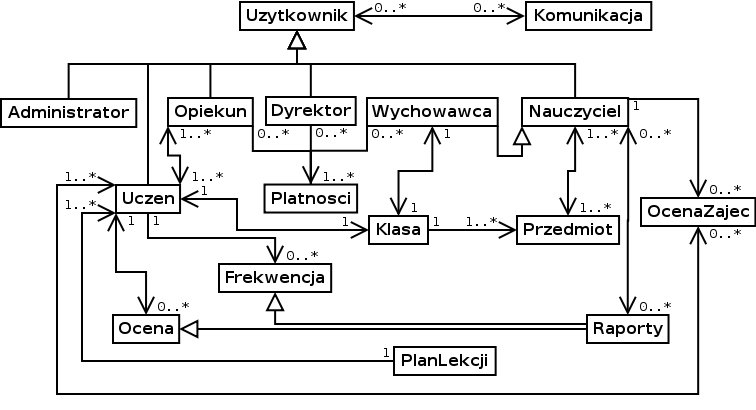
\includegraphics[width=16cm]{uml_klas.png}
\caption{Diagram UML}
\label{fig:uml}
\end{figure}

\subsection{Perspektywa implementacyjna}
\noindent Perspektywa implementacyjna skupia się na ustaleniach co do sposobu kodowania, implementowania projektu WiDz. Najważniejsze klasy i~zależności pomiędzy nimi zostały już zaprezentowane w~poprzednim podrozdziale, zatem tutaj skupimy się głównie na samym środowisku, w~którym będzie tworzony program.

%\indent Aby WiDz był produktem najwyższej jakości, cały proces implementacji będzie opierał się na programowaniu sterowanym zachowaniem\footnote{zob. \url{http://behaviour-driven.org/}} (ang. BDD --- \textit{Behavior-Driven Development}), przy użyciu biblioteki RSpec\footnote{biblioteka BDD dla aplikacji języka Ruby, zob. \url{http://rspec.info}}. Jest to podejście, które skupia uwagę programisty na 

\indent Aby WiDz można było uznać za produkt najwyższej jakości, po każdym etapie implementacji nawet najmniejszego fragmentu kodu, cały program powinien być testowany i~uruchamiany w~środowisku bardzo zbliżonym do tego, w~którym będzie eksploatowany po zakończeniu nad nim prac. W~tabeli \ref{elementy_architektury} dla przypomnienia prezentujemy istotne oprogramowanie, biblioteki oraz języki programowania użyte w~projekcie WiDz.

\indent Konfiguracja poszczególnych komponentów architektury została dopasowana do programu WiDz, by końcowy efekt był zgodny z~wymaganiami postawionymi w~dokumencie~\cite{WYM}. Struktura samej bazy danych odpowiada w~dużej mierze koncepcji klas, które zaprezentowano w~poprzednim podrozdziale.
\begin{table}[h]
	\centering
	\caption{Elementy architektury}
		\begin{tabular}{|l|p{10cm}|}
		\hline
		\textbf{Element architektury} & \textbf{Oprogramowanie, języki programowania} \\ \hline
		Serwer & HTTP Apache + moduł Passenger, rama Ruby on Rails, menadżer pakietów RubyGems \\ \hline
		Baza danych & SZBD MySQL na serwerze \\ \hline
		Pliki źródłowe & język Ruby, rama Ruby on Rails \\ \hline
		Interfejs użytkownika & witryna internetowa, języki HTML, CSS, JavaScript \\ \hline
		\end{tabular}
	\label{elementy_architektury}
\end{table}

\subsection{Perspektywa procesowa}
\noindent Poważnym problemem z~jakim może spotkać się WiDz, jest jednoczesna obsługa nawet kilkuset użytkowników, którzy w~tym samym momencie będą korzystać z~programu. Zdecydowana większość procesów jest uruchamiana po stronie serwera, dlatego WiDz musi skupić się na optymalnym wykorzystywaniu zasobów, którymi dysponuje, a także szukaniu sposobu na odciążenie serwera od nadmiaru pracy, wykorzystując przy tym klienta. 

\subsection{Perspektywa wdrożeniowa}
\noindent Aby wdrożyć program WiDz, należy wykonać następujące czynności:
\begin{enumerate}
	\item instalacja i~konfiguracja na serwerze oprogramowania serwerowego \hbox{HTTP Apache} + moduł Passenger, interpretera języka Ruby, menadżera RubyGems, ramy projektowej Ruby on Rails oraz podstawowych bibliotek\footnote{instalowane za pomocą menadżera RubyGems, są to moduły: dbi, erector, god, json, mysql, net-ssh, rails, rake, rspec} dedykowanych do użytku w~środowisku Ruby on Rails,
	\item instalacja i~konfiguracja na serwerze SZBD MySQL,
	\item skopiowanie źródeł WiDz na serwer,
	\item integracja programu WiDz z~SZBD MySQL i~oprogramowaniem serwerowym,
	\item instalacja i~konfiguracja programu GOD\footnote{GOD - program wspierający monitoring procesów uruchomionych na serwerze, dba o ich ciągłą obecność w~systemie},
	\item uruchomienie procesu dbającego o tworzenie codziennie kopii bezpieczeństwa danych w~bazie danych.
\end{enumerate}

\section{Architektura a cechy projektu WiDz}
\subsection{Efektywność}
\noindent Wykorzystując pamięć podręczną po stronie użytkownika do składowania tymczasowych danych, odciążamy serwer od nadmiaru zadań do wykonania, przerzucając ich część na użytkownika.
 
\subsection{Stabilność}
\noindent Język Ruby to bardzo popularny język, ciągle rozwijany, mający wielu zwolenników ze względu na ramę projektową Ruby on Rails. Bardzo rozbudowana biblioteka do testowania RSpec\footnote{biblioteka BDD (ang. BDD --- \textit{Behavior-Driven Development}) dla aplikacji języka Ruby, umożliwia pisanie testów jednostkowych, opisujących konkretne obiekty, jak i~testy w~postaci historyjek opisujących zadania, jakie powinna wykonać aplikacja } pomaga tworzyć testy dokładnie odpowiadające specyfikacji projektu, przez co wyłapywanie błędów i~ich naprawa odbywa się bardzo szybko. Ciągły rozwój użytych technologii w~WiDz sprawia, że program będzie zawsze zgodny z~najnowszymi wersjami systemów operacyjnych.

\subsection{Wygoda obsługi}
\noindent Przejrzysty, intuicyjny interfejs sprawia, że użytkownik nie ma problemów z~swobodnym korzystaniem z~programu WiDz. Wykorzystany język HTML, CSS, JavaScript pozwala na przyjazną interakcję z~użytkownikiem przy pomocy przeglądarki internetowej. Bez względu na używany system operacyjny, program zawsze wygląda tak samo. Stworzenie programu jako aplikacji internetowej pozwala na korzystanie z~niego z~dowolnego miejsca na ziemi.

\subsection{Możliwość rozwoju}
\noindent Wykorzystany w~WiDz wzorzec projektowy MVC daje duże możliwości, by w~prosty sposób rozszerzyć podstawowe funkcje programu o nowe działania. Mamy możliwość przeistoczenia dziennika elektronicznego w~program, który obok pierwotnych funkcji, oferowałby funkcje przydatne w~zarządzaniu placówką szkolną, np. zautomatyzowany przepływ dokumentów pomiędzy osobami, szkołą a ministerstwem.

\indent Informatyzacja w~tej dziedzinie jest niezbędna, by w~przyszłości proces kształcenia był bardziej efektywny.

\section{Słownik}
%\begin{itemize}
%\item BDD
%\item CSS
%\item HTML
%\item JavaScript
%\item MVC
%\item środowisko developerskie
%\end{itemize}
\noindent Słownik terminów użytych w~dokumencie znajduje się w~\cite{SLO}.

\begin{thebibliography}{99}
\bibitem{SP} Edward Benson, {\it RAILS Sztuka Programowania}. Gliwice, Wydawnictwo HELION 2009.
\bibitem{WYM} Michał Kopacz, Mateusz Nahalewicz, Karol Bajko, {\it Dokumentacja projektu WiDz -- Wirtualny Dziennik. Specyfikacja wymagań}. Wrocław, SPIO IIUWr 2009.
\bibitem{SLO} Michał Kopacz, Mateusz Nahalewicz, Karol Bajko, {\it Dokumentacja projektu WiDz -- Wirtualny Dziennik. Słownik}. Wrocław, SPIO IIUWr 2009.
\end{thebibliography}

\end{document}
